
\catcode`\&=12
\chapter{Introduction\label{H1Introduction}}
\section{What is HepODBMS?}
\index{CERNLIB}%

\par

HepODBMS is a C++ class library that provides a simplified and consistent
interface to underlying ODMG-compliant Object Databases (ODBMS).
It provides high-level clustering and locking strategies, simplifies database
session and transaction control and offers features important to HEP applications,
such as highly scalable event collections and event tags (``Ntuple'' replacement).

\par

The current implementation of HepODBMS is based upon Objectivity/DB. A basic
knowledge of Objectivity/DB concepts and terminology is therefore
assumed. Further details regarding Objectivity/DB can be found
\url{http://wwwinfo.cern.ch/asd/lhc++/Objectivity/index.html}.

\par

The goals of HepODBMS can be summarised as follows:

\begin{itemize}

\item Provide an insulation layer to minimize dependencies on a given
database vendor or release.
\item Provide high level base classes that encapsulate features such
as clustering and locking strategies, database session and transaction
control, event collections, selection predicates, tagDB access and
calibration.
\item Achieve the above whilst not introducing any significant
performance or storage overhead.\end{itemize}

\par

HepODBMS is composed of a number of packages. These are as follows:
\begin{DLtt}{Persistent Helper classes}
\item[Insulation Layer]A set of header files providing a release-independent interface
to the most commonly-used subset of the Objectivity/DB API.
\item[Transient Helper classes]A high-level, simplified interface to the database.
\item[Persistent Helper classes]Object clustering and naming and other utility classes.
\item[Tags and Collections]Tag, event collections and selection classes.
\item[Miscellaneous]Timers, statistics, TCL application class and so forth.
\item[Conditions DB]A ``calibration'' or ``conditions'' DB subpackage.
\end{DLtt}

\par

Before we describe these sub-packages in more detail, we first introduce a number of basic concepts.
\section{Basic Concepts}

\par

In this section, we introduce a few essential concepts that need to be understood
in order to work with an ODBMS such as Objectivity/DB. A more detailed discussion of
Objectivity/DB can be found in the Objectivity Technical Overview, available via
\url{http://wwwinfo.cern.ch/asd/lhc++/Objectivity/TechOver/index.htm}.

\par

An Objectivity/DB \emph{federated database} consists of:

\begin{itemize}

\item A \emph{bootfile}
\item A database catalogue (the \emph{federation})
\item One of more database files\end{itemize}

\par

A \emph{bootfile} is simply a small configuration file that points
to the real location of the federation and contains a number of other
parameters, explained later.
\par

The database catalogue contains the names and locations of all
of the databases making up that particular federated database. 
Each database is specified by the full pathname and filename and hostname on which
it resides. In addition, the catalogue contains the class definition, or \emph{schema},
of all objects that reside in the database. Before an object can be stored in the database,
the corresponding class definition must be defined in a step called \emph{schema processing}.

\par

In fact, each database also has internal structure, but this we defer until later.

\par

In order to work with a federated database, an application must first
initialise a \emph{database session}. For CERNLIB users, this
can be considered equivalent to a call to the HBOOK or ZEBRA
initialisation rountines, \Lit{HLIMIT} or \Lit{MZEBRA}
respectively.

\par

Databases process data in units of work called \emph{transactions}. Transactions
are a fundamental technique for providing consistency. Either all of the changes that
form part of a transaction are made - if the transaction successfully \emph{commits},
or none are - if it \emph{aborts}. This is true for both reading and writing - a
transaction must be started before a single object is read from the database. This
allows the database to ensure that the application sees a consistent state, regardless
of changes being made concurrently by other users.

\par

Thus, the simplest database application would perform the following steps:

\begin{itemize}

\item Initialise.
\item Start a transaction (in read or update mode).
\item Read or write one or more objects.
\item Commit the transaction and terminate.\end{itemize}

\par

These steps are shown in the following code fragment.
\begin{verbatim}
#include "HepODBMS/clustering/HepDbApplication.h"
    HepDbApplication myApp("MY_FDB"); 
    // initialize db connection 
    myApp.Init();        // initialise the db session 
    // start an update transaction if you are going to write to a database 
    myApp.startUpdate(); // start an update transaction 
    ---- work with the objects in a database ------------ 

    // commit all changes made during this transaction 
    myApp.commit(); 

\end{verbatim}
\section{The Storage Hierarchy of Objectivity/DB}

\par

As described above, Objectivity/DB supports a so-called \emph{federated
database}, which is a single, logical database composed of up to
65536 \emph{physical databases}.  Each physical database is
simply a file, stored on a specified host. The physical databases - or
files - consist of \emph{database pages} in which the persistent
objects are stored. The size of each database page is constant within
a given federation and can vary between 512 bytes and 64KB. Typical
values are 1KB - 8KB.

\par

\includegraphics[width=.7\linewidth, scale=.5]{fdb_structure}

\par

Between the database and page there is an additional layer, called a
\emph{container}.  Containers are sets of contiguous database
pages within a given file. As the unit of I/O in Objectivity/DB is always a
multiple of database pages, it is useful - for performance reasons -
to \emph{cluster} objects that are likely to be accessed
together on the same - or adajacent - pages. The concept of a
container provides a mechanism for performing such clustering at a
finer level than would be possible using simply files.
\section{Persistent versus Transient Objects}

\par

In a ``normal'' - i.e. \emph{transient} - C++ application,
objects are defined in C++ header files, created using the \Lit{new}
operator and then accessed using C++ pointers.

\par

In a persistent application - that is, one that uses ``database objects'',
one works with \emph{schema}, an enhanced (\emph{overloaded}) \Lit{new}
operator and ``smart pointers'', or ``references''. These are all
used in essentially the same way as in the transient case, as is shown in the following example.

\begin{verbatim}

// Transient example

// Persistent example

\end{verbatim}

\par

In addition to these small changes, it must be stressed that access to persistent
objects \emph{must} take place within a \emph{transaction},
which in turn must be within an active database session.
\par

Thus, before creating new persistent objects, or accessing existing ones, an application
must first initialise a database session and start a read or update transaction, as 
appropriate.
\par

In order for any changes to be made persistent, the corresponding transaction must 
\Lit{commit}. Simply terminating the process will result in an abort of any
outstanding transactions and the changes will \Lit{not} be made to the database.
\chapter{Getting Started\label{H1GettingStarted}}
\section{Introduction}

\par

In this section, we describe the basic building blocks of a persistent application.
These are:

\begin{itemize}

\item The HepODBMS insulation layer
\item The HepODBMS database interface
\item Schema processing\end{itemize}

\par

These three components will allow you to create an application that manipulates 
objects that you have defined.
\section{The HepODBMS Insulation Layer}

\par

As different releases of Objectivity/DB have small variations in the API, and in order
to provide the possibility of migration between underlying database systems -
an extremely important issue when dealing with timescales of the order of the LHC - 
it is \Lit{strongly} recommended that applications using the HepODBMS
insulation layer, rather than make direct calls to the Objectivity/DB API.

\par

The HepODBMS insulation layer consists of two parts:

\begin{itemize}

\item A set of fixed-length types, as defined by the ODMG
\item High-level interface classes to the database itself, and for
working with persistent objects.\end{itemize}

\par

Fixed-length types are required to support \emph{platform heterogeneity} - that is,
the possibility of storing objects on a machine of one architecture, such as
a Sun, and reading them back on another - perhaps a Digital Unix system.
As the native language types - \Lit{int, float} etc. - do not have
strict definitions, the ODMG introduces fixed length types, as shown
in the table below. These types should \Lit{always} be used as
data members of persistent objects, rather than the native types.

\begin{table}\centering
\caption{ODMG types and their meaning\label{tab-odmg}}

\par

\begingroup\catcode`\&=4
\begin{tabular}{ll}
\emph{ODMG type}&\emph{Definition}\\
\Lit{d_Short}&16bit signed integer\\
\Lit{d_Long}&32bit signed integer\\
\Lit{d_Short}&16bit unsigned integer\\
\Lit{d_UShort}&32bit unsigned integer\\
\Lit{d_ULong}&32bit IEEE float\\
\Lit{d_Float}&64bit IEEE float\\
\Lit{d_Double}&16bit signed integer\\
\Lit{d_Char}&8bit ASCII character\\
\Lit{d_Octet}&8bit - no interpretation\\
\Lit{d_Boolean}&0 or 1\\

\end{tabular}\catcode`\&=12\endgroup
\end{table}

\par
An example of the use of these fixed length types is shown below.
\begin{verbatim}
#ifndef Track_ddl 
     #define Track_ddl 
     #include "HepODBMS/odbms/HepODBMS.h" 
     class Track : public HepPersObj { 
     protected: 
       d_ULong   noOfHits; // value range of these fields 
       d_Double  theta;    // will be the same on all machines 
       d_Double  phi;      // 
     public: 
       Track() 
           :noOfHits(0),theta(0),phi(0) 
         { 
           // constructor does nothing yet... 
         } 
       d_Long    getNoOfHits { return noOfHits; } 
       d_Double  getTheta { return theta; } 
       d_Double  getPhi { return phi; } 
       static HepContainerHint clustering; 
     }; 
     #endif

\end{verbatim}

\par

Note that these types should only be used in connection with 
persistent objects. As is shown in the following example,
switching globally to these types is likely to cause problems on 
certain systems and should thus be avoided.
\begin{verbatim}
  const d_Long size = 10000; // the buffer size 
  char *buffer = malloc(size);
 // Error if d_Long is not the same as size_t!

\end{verbatim}
\section{Working with Persistent Objects}

\par

In order to work with persistent objects, classes to handle the database session and
transactions are needed, as well as classes to deal with databases, containers
and persistent objects themselves.

\par

The following classes are provided:\begin{DLtt}{HepContainerRef}
\item[HepRef]Equivalent to Objectivity/DB's \Lit{ooHandle} - objects are pinned 
in memory as long as the reference is being used.
\item[HepDatabaseRef]A reference to a database.
\item[HepContainerRef]A reference to a container.
\end{DLtt}

\par

There usage is shown in the following set of code fragments.
\begin{verbatim}

// start an update transaction 
  startUpdate(); 

  // create a db named "TrackData" or switch to it if it exists already 
  HepDatabaseRef mydb = db("TrackData"); 

  // create a container "TrackTables". If it exists already, just return the handle 
  HepContainerRef cont = container("TrackTables"); 

  // create 10 persistent track tables 
  for (int i=0; i<10; i++) 
  { 
    // create the persistent object (TrackTable) 
    HepRef(SimpleTrackTable) ttab = new(cont) SimpleTrackTable(i); 
  } 

\end{verbatim}

\par

In addition. two arrays are provided:
\begin{DLtt}{HepRefVector(T)}
\item[HepVector(T)]A wrapper to \Lit{ooVArray(T)}
\item[HepRefVector(T)]A vector of references
\end{DLtt}

\begin{verbatim}
//DDL files 
class Hit : public HepPersObject { 
public: 
d_Double q; //charge
}; 
class Track : public HepPersObj { 
public: 
d_ULong noOfHits; 
HepRef(Vertex) vtx; 
HepRefVector(Hit) hit;
}; 
\end{verbatim}

\begin{verbatim} 

//main example2.cpp file 
#include "HepODBMS/tagdb/HepTagDbApplication.h" 
#include "HepODBMS/tagdb/HepEvent.h" 
main() 
{ 

//start a session 
HepDbApplication dbApp; 
// define which federation to use 
dbApp.fdBootName("MyBase"); 
// open federation 
dbApp.Init(); 
// start in read mode 
dbApp.StartUpdate(); 
// switch to database "analysis" 
dbApp.db("analysis"); 
//creating objects and clustering them together by class 
HepRef(Track) aTrack = new Track; 
// dereferencing 
aTrack->noOfHits = 0; 
//double deref 
cout "vtx.x" << aTrack->vtx()->x << endl; 
// vector access 
cout "hit[0].q" << aTrack->hit[0].q << endl; 
// Commit all changed objects 
dbApp.Commit();
}

\end{verbatim}
\section{Schema Processing}

\par

Before an object can be stored in a database, its \emph{schema} or class definition
must be known. This is done using an Object or Data Definition Language (ODL or DDL).
The class definition is used by the database to ``reassemble'' 
an object when it is read back from the database - converting it from its persistent representation
to something understandable to the C++ run-time system. This includes not only converting
the data - as and when required by the system in question - but also rebuilding 
the table of methods associated with the object, so that they may be invoked just as
in the transient case.
\par

To a large extent, the schema of a given class is the same as the corresponding C++ header file.
The main differences are as follows:
\begin{itemize}

\item Persistent-capable objects must \Lit{inherit} from a special persistent base class.
The class provided by HepODBMS for this purpose is \Lit{HepPersObj}.
\item The use of C++ pointers and references must be replaced by ODMG ``smart pointers''.
\item The Objectivity/DB implementation
does not permit persistent-capable objects to be embedded in other persistent-capable
objects.\end{itemize}

\par

Schema processing in Objectivity/DB is shown in the following diagram.
\par

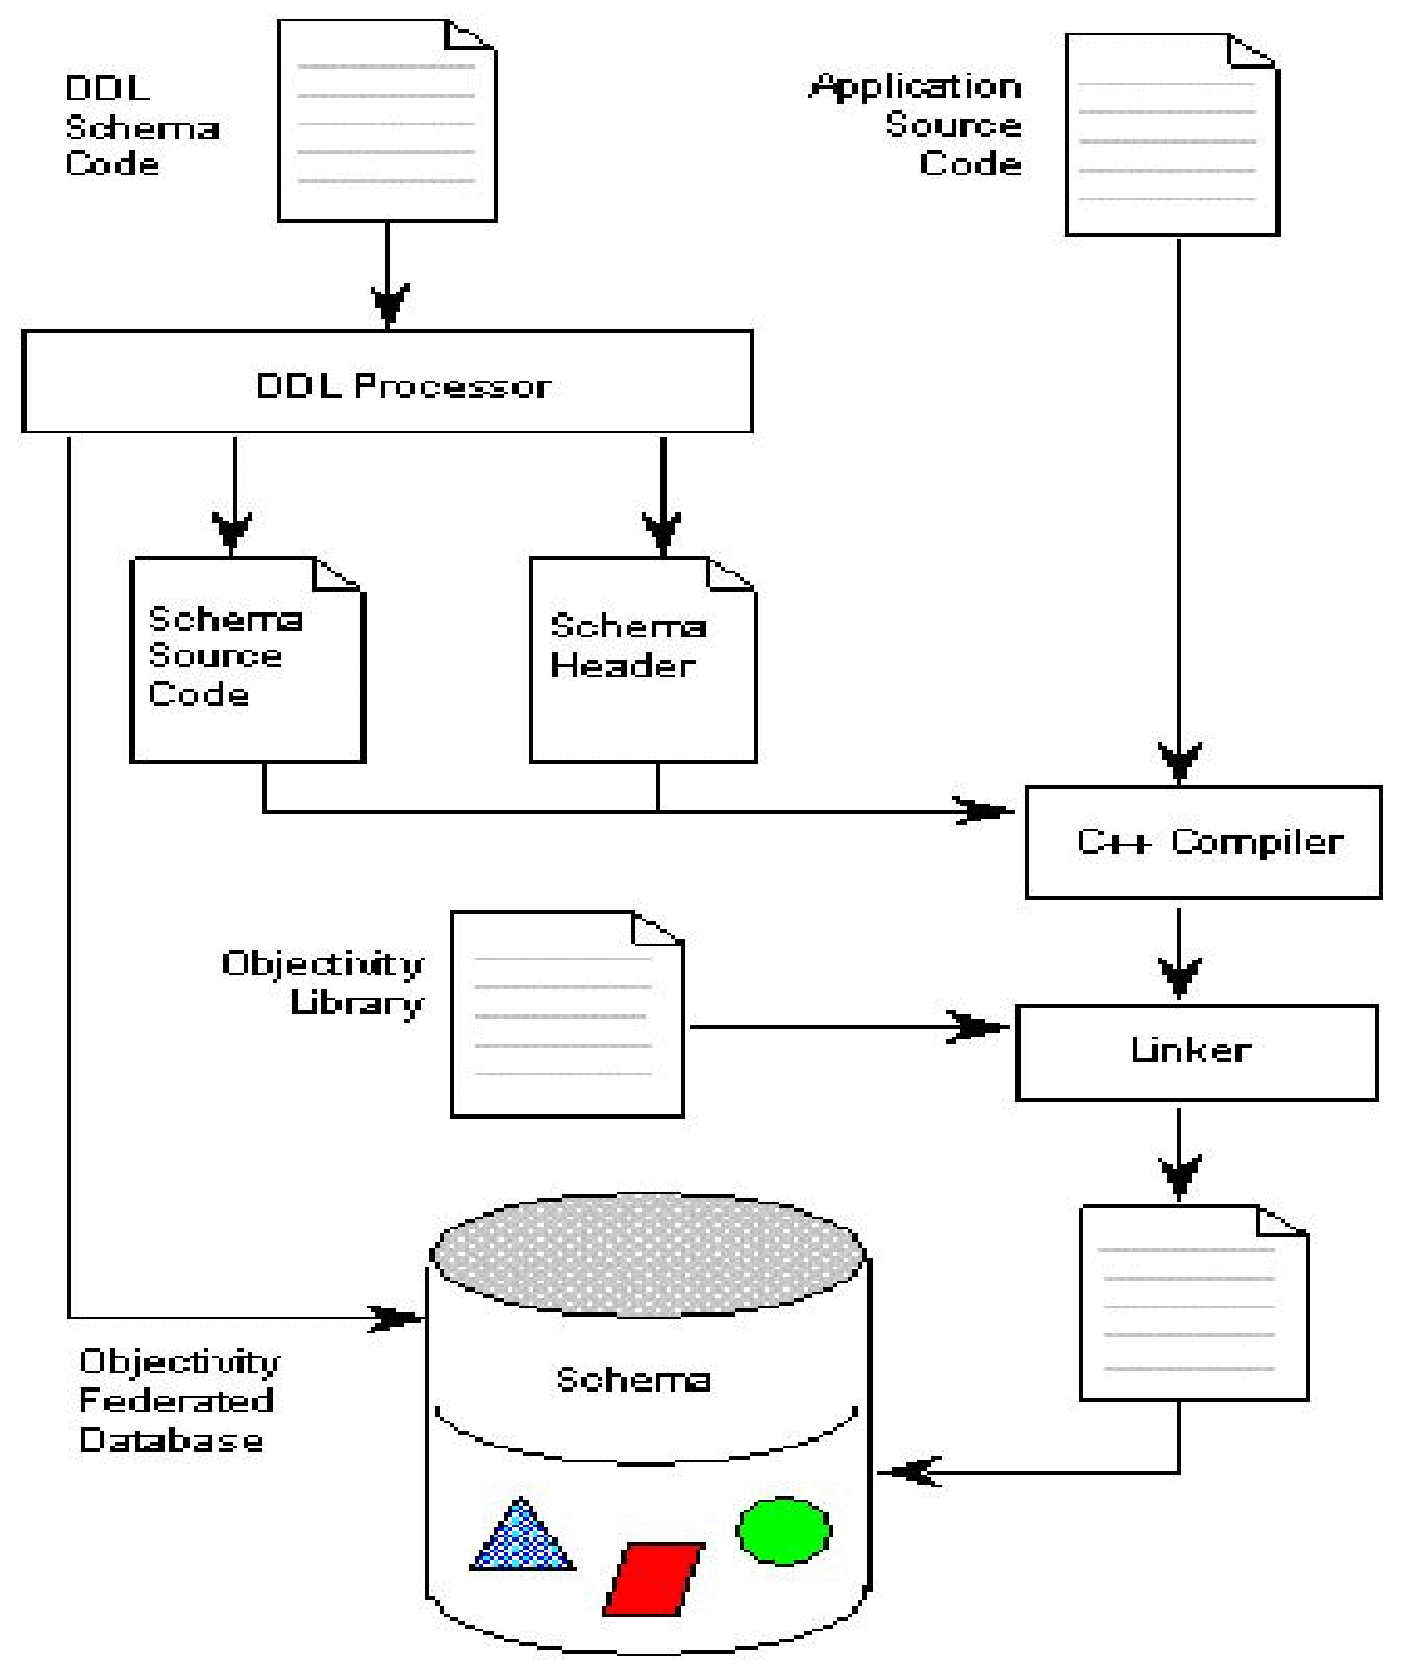
\includegraphics[width=.7\linewidth, scale=.5]{schema}

\par

The example below shows the definition of several persistent capable
objects: \Lit{Event}, \Lit{Tracker} and \Lit{Calo}.
All of these objects inherit directly from \Lit{HepPersObj}.
In addition, two transient objects, \Lit{Track} and \Lit{Cluster}
are made persistent \emph{by containment}. That is, they are embedded
in an object which is persistent capable and these embedded instances are
thus made persistent in their own right.

\par

Additional constructs with respect to pure C++ are also
possible. These include variable length arrays -
\Lit{d_Varray<T>} - and associations. Associations
may be single or bi-directional, 1-N or N-M.
\begin{DLtt}{d_Ref<Tracker> itsTracker <-> itsEvent;}
\item[d_Varray<Track> tracks]A variable length array (of tracks).
\item[d_Ref<Tracker> itsTracker <-> itsEvent;]A bi-directional association.
\item[d_Ref<Event> itsEvents[];]1-to-N or N-to-M associations.
\end{DLtt}

\begin{verbatim}
// File: /HepODBMS/examples/populateDb/Event.ddl 

#ifndef __EVENT_DDL 
#define __EVENT_DDL 

#include "HepODBMS/clustering/HepClusteringHint.h" 
#include "HepODBMS/clustering/HepContainerHint.h" 

// a simple track -  *not* peristent by itself but by 
// embedding it in the persistent tracker object 
  

class Track { 
public: 
  // default constructor: init members to 0 
  Track(): 
      phi(0),theta(0),pt(0) 
    {} 

  // constructor just assigns the datamembers 
  Track(double _phi, double _theta, double _pt): 
      phi(_phi),theta(_theta),pt(_pt) 
    { } 

  double getPhi()   { return phi;} 
  double getTheta() { return theta;} 
  double getPt()    { return pt;} 

private: 
  double phi; 
  double theta; 
  double pt; 
}; 
  

/// persistent Tracker class, contains a variable size array of Track objects 
class Tracker : public HepPersObj { 
public: 
  /// create a new Tracker object with an track list for 
  /// noOfTracks Tracks. 

  Tracker (long noOfTracks): // pass the size to the varray contructor 
      tracks(noOfTracks) 
    { /* nothing else needed */ } 

  long getNoOfTracks() { return tracks.size(); } 

  d_VArray<Track> tracks; 

  static HepContainerHint clustering; 
private: 
}; 
  

class Cluster { 
public: 

  Cluster() : energy(0), theta(0), phi(0) 
    { /* nothing else needed */ } 

  Cluster(double _phi, double _theta, double _energy): 
      phi(_phi), theta(_theta), energy(_energy) 
    { /* nothing else needed */ } 
  

  double getPhi()    { return phi; } 
  double getTheta()  { return theta; } 
  double getEnergy() { return energy; } 

private: 
  double phi; 
  double theta; 
  double energy; 
}; 

/// persistent Calo class, contains a variable size array of Cluster objects 
class Calo : public HepPersObj { 
public: 
  Calo(int noOfClusters): 
      clusters(noOfClusters) 
    { /* nothing else needed */} 

  int getNoOfClusters() 
    { return clusters.size(); } 

  d_VArray<Cluster> clusters; 

  static HepContainerHint clustering; 
}; 

/// persistent Event class 
class Event : public HepPersObj { 
public: 
  Event(int no): 
    evtNo(no) 
    { /* nothing else needed */} 

  int getEventNo() { return evtNo;} 

private: 
  int evtNo; 

public: 
  d_Ref<Tracker> tracker; 
  d_Ref<Calo>    calo; 

  static HepContainerHint clustering; 
  
}; 

#endif /* __EVENT_DDL */ 

\end{verbatim}
\chapter{Clustering and Naming\label{H1ClusteringNaming}}
\section{Object Clustering}

\par

The ODMG standard states that a ``clustering hint'' may be specified
(as an argument to the \Lit{new} operator), when persistent objects
are created. This is done by passing a reference to another object - 
such as the previous object of this type that was created. The new
object is then created at a physical location that is ``close''
to the previous one. This might be on the same database page - if there
is sufficient room - or the next free one.
\par

In Objectivity/DB, clustering works at the level of \emph{containers}. As this is
also the level at which locking works in Objectivity/DB, there are two issues that we need
to consider:
\begin{itemize}

\item A way to minimise lock contention when multiple processes are
reading or writing to the same federation.
\item The possibility of providing logical clustering that is not limited
by the physical capacity of an individual container (64K logical pages).\end{itemize}

\par
Both of these issues are addressed in HepODBMS.
\par
A typical clustering strategy might be to store all objects of a given class in the same ``logical''
container. In the case of a class such as a \Lit{Track}, a single container would clearly
be inadequate for this purpose. The HepODBMS clustering classes permit such ``class-based'' clustering,
automatically creating new containers as required. This is shown in the following example.

\begin{verbatim}
  // define a reference to a container 
 HepContainerRef trackContainer; 
 // initialise the container ref 
 // ... 
 // create 100 tracks clustered together 
 // in the container "trackContainer" 
 for (i=0; i<100; i++) 
 // specify the track container as clustering hint for the new track 
 HepRef(Track) aTrack = new(trackContainer) Track;

\end{verbatim}

\par

The simplest concrete class provided by the library is the \Lit{HepContainerHint}. 
Objects of this class simply return as a hint the reference to a container that has been set e.g. at program startup. 
This is shown in the following code fragment.
\begin{verbatim}
// create and init the hint at prg startup 
HepContainerHint trackClustering = dbApp.container("Tracks")
    // any track creation looks like this 
    HepRef(Track) aTrack = new (trackClustering::getHint()) Track; 

\end{verbatim}

\par

If all the objects of a given class share the same hint, one convenient way to define 
the clustering hint is to put it as a static member in the class definition. 
(Static members are instantiated only once, are accessible from all objects of the class and are not stored in the database). 
This is shown below.
\begin{verbatim}
 /// persistent Event class 
class Event : public HepPersObj { 
public: 
  Event(int no): 
    evtNo(no) 
    { /* nothing else needed */} 
  int getEventNo() { return evtNo;} 

private: 
  int evtNo; 

public: 
  d_Ref<Tracker> tracker; 
  d_Ref<Calo>    calo; 

  static HepContainerHint clustering; 

};
\end{verbatim}

\par
 
The static member clustering has to be allocated (e.g. in a .cpp file) using a statement like:

\begin{verbatim}
    // allocate static variables 
    HepContainerHint Event::clustering; 
\end{verbatim}

\par
This variable must
be initialised before it is first used e.g. using:
\begin{verbatim}
     db("Events"); 
     Event::clustering = container("EventsCont"); 
\end{verbatim}

\par

New \Lit{Event} objects are now created using:
\begin{verbatim}
HepRef(Event) evt = new( Event::clustering() ) Event(i);
\end{verbatim}

\par
Note the use of the operator() shortcut for the getHint() method.
\par

For convenience a \Lit{HepNew} macro is provided. This performs
the same function as the above, but hides the additional argument for the new operator.
\begin{verbatim}
HepRef(Event) eventRef = HepNew(Event);
\end{verbatim}

\par

The following example demonstrates the usage of class-based clustering.
Although the creation of new objects of type \Lit{Track} may be
spread throughout the entire code, the definition of the clustering
hints is performed in a single place, and can thus be much more easily controlled.

\begin{verbatim}
//
// Class Based Clustering
//
// class definition in Track.ddl 
class Track : public HepPersObject 
{ 
d_Double phi; 
d_Double theta; 
d_ULong noOfHits; // more stuff 
public: 
static HepContainerHint clustering;
}; 
... 

// clustering definition at startup 
Track::clustering = dbApp.container("tracks"); 
// clustering use spread all over the source code 
HepRef(Track) aTrack = new (Track::clustering()) Track;

\end{verbatim}

\par

(Note the use of the scope resolution operator \Lit{::} to access the class member).
This other examples shows you how to make persistent Clustering in Parallel Writers: 
\begin{verbatim}
//
// Example of parallel writing
//
// class definition in Track.ddl 
class Track : public HepPersObject { 
d_Double phi; 
d_Double theta; 
d_ULong noOfHits; // more stuff 
public: 
static HepClusteringHint clustering;
}; 
// read or create persistent clustering definition at startup 
if (!Track::clustering.find("tracks")) 
Track::clustering.create("tracks")); 
Track::clustering.setParallelWriterMode(noOfProcs,myID); 
// clustering use spread all over the source code 
HepRef(Track) aTrack = new (Track::clustering()) Track; 

\end{verbatim}
\section{Object Naming}

\par

Any persistent object that is stored in the database may be given a \emph{name}.
A name is simply a text-string that is associated with an object. Of course, it is 
not intended that \emph{every} object in the database is named - this would not be 
efficient and would have a significant overhead. Naming is most useful for defining
``entry points'' into the database. For example, a collection of events could be
given a name - such as ``Higgs candidates''. As a flat naming scheme is often inadequate
- and would clearly not be useful in a multi-user system, HepODBMS provides a hierarchical
naming scheme, similar to that of a Unix filesystem.

\par
The \Lit{HepNamingTree} class provides the following Unix-like methods:

\begin{itemize}

\item makeDirectory(path), 
\item changeDirectory(path), 
\item removeDirectory(path), 
\item nameObject(objRef,path), 
\item findObject(path), 
\item removeName(path), 
\item removeObject(path), 
\item startItr(), 
\item nextItr() \end{itemize}

\par

The usage of these methods is shown in the following example. The
\Lit{HepDBApplication} class automatically places the application
in the ``directory'' corresponding to the current username, to
avoid possible conflicts between the naming trees of different users.
Naturally, it is possible to navigate to any point in the naming tree.

\begin{verbatim}
typedef h_seq<Event> EventCol; 

// initialize DB session 
HepDbApplication app; 
app.init("fdBootName"); // implicit cd /usr/$USER/ 
// move to test-beam 
app.naming.changeDirectory("test-beam"); 
evtCol = EventCol::findByName("inputEvents"); 
EventCol::iterator it; 
for (it = evtCol.begin(); it != evtCol.end(); it++) 
{ 
    -- do something-- 
}
\end{verbatim}
\chapter{Collections and Tags\label{H1CollectionsTags}}
\section{STL Collections}

\par

The C++ standard includes the definition of a set of collections based upon the work
of Alex Stepanov and Meng Lee. These collections are frequently referred to as
the ``Standard Template Library'' or STL, although the more correct
term is simply the Standard Library.

\par

The ``STL'' includes the following:\begin{DLtt}{Allocators}
\item[Containers]Generalized classes used to hold a collection of typed data.
\item[Iterators]Generalized pointers used to traverse the elements of a container.
\item[Algorithms]Procedures that can be applied on all or part of a container.
\item[Function Objects]Behaviors used as a parameter by a container or algorithm.
\item[Allocators]Objects responsible for allocating storage.
\end{DLtt}

\par

More information on the STL can be found via the following URL:
\url{http://wwwinfo.cern.ch/asd/lhc++/ObjectSpace/doc/2.1/index.html}
\par

The following example shows the use of STL collections.
\begin{verbatim}
#include <iostream> 
#include <vector> 
int array[] = { 1, 42, 3 }; // Regular "C" array. 
vector < int > v; // STL transient vector of integers 

int main() 
  { 
  // Initialize the STL Vector 
  v.push_back( 1 ); 
  v.push_back( 42 ); 
  v.push_back( 3 ); 

  // Use pointer to traverse "C" array. 
  int* p1; 
  for ( p1 = array; p1 != array + 3; ++p1 ) 
    cout << "array has " << *p1 << "\n"; 

  // Use iterator to traverse STL vector. 
  int_vector::iterator p2; 
  for ( p2 = v.begin(); p2 != v.end(); ++p2 ) 
    cout << "vector has " << *p2 << "\n"; 
  } 
    return 0; 
 } 
 
\end{verbatim}

\par

The ODMG standard includes STL-compliant collection classes. For
the main STL collections, a persistent equivalent exists, designated
by a leading \Lit{d_}.

\par

Objectivity/DB provides persistent STL collections classes based upon the 
ObjectSpace implementation - also available in transient form
via LHC++.
\par

The following example demonstrates the use of persistent STL collections.
\begin{verbatim}

// Example of persistent STL

\end{verbatim}
\section{HepODBMS Collections}

\par

In addition to the persistent STL collections described above,
HepODBMS provides highly scalable collections - capable of handling
very large numbers of entries. They were designed to handle up to
1000 million objects, which would not be possible using the
standard persistent STL classes offered with Objectivity/DB.

\par
 HepODBMS defines following templated collection that is usable for any kind of persistent objects:
\par
\Lit{typedef h_seq<Event> EventCollection;}
\par

The interface of this collection offers the following: 
\begin{itemize}

\item STL interface independent of implementation.
\item Single User visible collection class : \Lit{h_seq<T>}
\item Single STL like iterator: \Lit{h_seq<T>::iterator}
\item Uses hybrid of templated classes and delegation.
\item User extensible through strategy objects.\end{itemize}

\par

For example, we may wish to access an existing event collection
by name. We first define the collection, as follows:
\par
\Lit{EventCollection evtCol("/usr/dirkd/collections/myEvents");}
\par
We then need to define an \emph{iterator} for this collection (STL-like):
\par
\Lit{EventCollection::const_iterator it;}
\par
We can now iterate through the collection and read individual
event objects:
\begin{verbatim}
it = evtCol.begin(); 
while( it !=  evtCol.end() ) 
    { 
 cout << "Event: " << (*it)->getEventNo() << endl; 
     ++it; 
    } 
// support for (some) STL algorithms 
 int cnt=0; 
 count(evtCol.begin(),evtCol.end(),1,cnt);

\end{verbatim}

\par
Writing to the collection - e.g. adding new events - is shown below.
\begin{verbatim}
HepRef(Event) evt; 
for (int i=0; i<500000; i++) 
    { 
    // create a new event using the clustering hint of the sequence 
    evt = new(evtCol.clustering()) Event; 
  
    // store the new object ref in the sequence (only needed for ref collections) 
    evtCol.push_back(evt); 

    // fill the event 
    evt->setEventNo(i); 
  }
\end{verbatim}

\par

The following example shows how the HepODBMS collection
class may be used to store events. It is available
via  /afs/cern.ch/sw/lhcxx/share/HepODBMS/examples/createCollection/createCollection.cpp 

\begin{verbatim}
#include "HepODBMS/clustering/HepDbApplication.h" 

#include "EventSeq.h" 

d_Ref<ooObj> VStore<Event>::store_clustering; 

void print_evt(d_Ref<Event> evt) 
{ 
  cout << "Event Nr=" << evt->getEventNo() << endl; 
} 
  

int main(int argc, char *argv[]) 
{ 
  // 
  // Persistent event collection tests. 
  // 
  HepDbApplication app; 
  
  app.init(); 
  
  app.startUpdate(); 

  ooHandle(ooDBObj) db_h = app.db("Sequences"); 
  ooHandle(ooContObj) ooc_h; 
  
  ooHandle(ooContObj) eventCont = app.container("Events"); 
  ooc_h= app.container("Stores"); 

  ooDelete(eventCont); 
  ooDelete(ooc_h); 

  VStore<Event>::store_clustering = app.container("Stores",1); 
  eventCont = app.container("Events"); 
  app.commit(); 

  cout << "created db and container" << endl; 

  app.startUpdate(); 
  
  h_seq<Event> seq("dirks","vector"); 

  app.commit(); 
  cout << "created store object" << endl; 
  app.startUpdate(); 

  HepRef(Event) evt; 

  for (int i=0; i<5000; i++) 
  { 
    // create a new event, use the clustering hint of the sequence 
    evt = new(seq.clustering()) Event(i); 
  
    // store the new object ref in the sequence (only needed for ref collections) 
    seq.push_back(evt); 

  } 

  app.commit(); 

  return 0; 
}
\end{verbatim}
\section{Event Tags}

\par
An \emph{event tag} (or rather a collection of such tags)
can be thought of as something similar to an Ntuple or an event directory.
Just as event directories are used to speedup event selection, tags
are introduced to speed up analysis - or indeed and other process
in which events are first selected. A tag may contain only information
relevent to the selection process itself - the data that is then used in the
analysis being obtained from other objects ``connected'' to the tag
via associations, or both the data used for selection and subsequent analysis (Ntuple-style).

\par
Two types of tags are provided, sharing a common interface. These are
as follows:\begin{DLtt}{Concrete tags}
\item[Generic tags]No schema definition is required.
\item[Concrete tags]Schema processing necessary.
\end{DLtt}

\par
Generic tags are aimed at ``not too large'' collections, typically owned by individual users. 
They provide a simple user interface for creation of tag quantities and eliminate the 
inconvenience for the end user to formally define a new persistent class when the set of user quantities changes. 
Generic tags may contain attributes of type float, double, short, long, char. 
Additional attributes may be added after the initial definition. 
This flexibility makes the generic tag particularly useful during the first development 
phase of an analysis, when the set of quantities used in the analysis tends to change more frequently. 
Although they carry a slight performance penalty with respect to concrete tags, 
they are more convenient for end users and avoid any schema handling issues.

\par
As the interface to both generic and concrete tags is identical, the examples
below concentrate on the generic tags.
\par

A new tag collection is defined as follows:
\par
\Lit{GenericTag highPt("high pt events"); }
\par
Tag attributes can now be defined and filled just like other C++ variables: 
\begin{verbatim}

TagAttribute<long>   evtNo(highPt,"eventNo"); 
TagAttribute<double> ptPlus(highPt,"ptPlus"); 
TagAttribute<long>   nTracks(highPt,"nTracks"); 
if (highPtTracks > 2) 
{ 
 // create a new tag and store the event reference 
 highPt.newTag(evt); 

 // define its tag attributes 
 evtNo   = evt->eventNo; 
 ptPlus  = evt->tracker.tracks[plusTrack].pt; 
 nTracks = evt->tracker.tracks.size();

\end{verbatim}

\par

The following example shows the creation and filling of a tag collection.
\begin{verbatim}

// File: HepODBMS/examples/createTag/createTag.cpp 

#include "HepODBMS/tagdb/HepAnalysis.h" 

#include "Event.h" // generated with ooddlx from Event.ddl 

class createTagsApp : public HepTagDbApplication { 
  // inherits session control from HepTagDbApplication 
  
public: 
  // this application implements just one method: 
  int run() 
  { 

    const char *tagName="high pt events"; 
    cout << "*** creating a tag collection" << endl; 

    startUpdate(); // start an update transaction 

    HepExplorable *cd = HepExplorable::findExplorable(tagName); 
    if (cd) { 
      cout << "removing old tag:" << tagName << endl; 
      cd->removeDescription(); 
      delete cd; 
    } 
  

    HepExplorableGenericTags highPt; // create a tag collection 
    db("Tags"); 

    if (!highPt.createDescription(tagName)) // start creating a new field description 
      fatal("could not create new tag");  // print the message and stop the application 

    // define fields all fields that belong to genTag 
    TagAttribute<long>  eventNo (highPt,"eventNo"); 
  
    /* track 1*/ 
    TagAttribute<double> ptPlus (highPt,"ptPlus"); 
    TagAttribute<double> phiPlus(highPt,"phiPlus"); 
  
    /* track 2*/ 
    TagAttribute<double> ptMinus (highPt,"ptMinus"); 
    TagAttribute<double> phiMinus(highPt,"phiMinus"); 
  

    cout << endl; 

    db("Events"); 
    ooItr(Event) eventItr; 
    eventItr.scan(container("Events")); 

    HepRef(Event) evt; 
    // now fill some tags 
    while( eventItr.next()) 
    { 
      // check for opposite signed pt > 5 
      HepRef(Tracker) aTracker = eventItr->tracker; 

      // keep index to current largest pt for each sign 
      int maxTrack = 0; 
      int minTrack = 0; 

      for (int track=0; track < aTracker->getNoOfTracks(); track++) 
      { 
        if (aTracker->tracks[track].getPt() 
            > aTracker->tracks[maxTrack].getPt() ) 
          maxTrack = track; 

        if (aTracker->tracks[track].getPt() 
            < aTracker->tracks[minTrack].getPt() ) 
          minTrack = track; 
      } 
  
      highPt.newTag();      // create a new tag (all fields have default values) 
      eventNo  = eventItr->getEventNo(); 
  
      ptPlus   = aTracker->tracks[maxTrack].getPt(); 
      phiPlus  = aTracker->tracks[maxTrack].getPhi(); 

      ptMinus  = aTracker->tracks[minTrack].getPt(); 
      phiMinus = aTracker->tracks[minTrack].getPhi(); 
  
    } 
    // commit this transaction 
    commit(); 
    return 0; 
  } 
}; 

int main() 
{ 
  createTagsApp myApp;  // create an application object 
  myApp.init();        // initialise the db session 
  return myApp.run();   // run it 
} 
\end{verbatim}
\chapter{Conditions Database\label{H1ConditionsDatabase}}
\section{Introduction}

\par
This section describes a ``conditions'' or ``calibration''
database application library, built on top of Objectivity/DB. It is based upon the
conditions database application, built by Jim Onhemus for the BaBar experiment.
The user guide for the BaBar library can be found 
\url{http://wwwinfo.cern.ch/asd/lhc++/HepODBMS/user-guide/docs/ConditionsDBapi.ps}.

\par

The basic purpose of this library is to store detector-related information
with an associated ``validity period'' and allow retrieval based upon a
validity instant. A typical example is the storage and retrieval of detector
calibration information. As such, the application must support multiple entries
for the same or overlapping validity period and provide flexible mechanisms for
retrieving the desired data.
\section{Storing and Retrieving Information}

\par

The interface to the conditions database is built on a small number of classes. These are as 
follows:\begin{DLtt}{HepCalibApplication}
\item[HepCalibApplication]Handles database sessions and transactions
\item[HepCalibDatabase]Used to create new calibration databases
\item[calibInterval]Used to store calibration information and associated validity period
\end{DLtt}

\par

The use of these classes is illustrated in the following code fragments.
The first demonstrates the use of the \Lit{HepCalibApplication} class.
\begin{verbatim}
// initialize the federated database 
  calibApp = new HepCalibApplication(fdBootName); 
  
  // start transaction for update 
  calibApp->startUpdate(); 
   --- work with the calibration database ---- 

     // save changes on disk 
   calibApp->startUpdate();
\end{verbatim}

\par

The use of \Lit{HepCalibDatabase} is shown below.
\begin{verbatim}
theDatabase = new HepCalibDatabase ( calibApp, "cal", dbPathName); // create calibration database group system 

theDatabase->open (); // open the database
\end{verbatim}

\par

The above code fragment will create a directory \Lit{cal} under the directory
specified by \Lit{dbPathName}. When such a directory is created, two database
files are automatically generated. These are \Lit{cal00000.DB} and \Lit{IndexCal.DB}.
The first file contains the calibration constants themselves. The calibration database system
will automatically create new files (cal00001.DB, cal00002.DB, ...) as required. The file
\Lit{IndexCal.DB} contains the validity instants for all inserted calibrations.
The calibrations themselves can be any persistent C++ object.

\begin{verbatim}
// Define a time interval ( theBeginTime, theEndTime ) 
HepTime theBeginTime = HepTime( 1996, 1, 1, 0, 0,  10 ); 
HepTime theEndTime =  HepTime( 1996, 1, 1, 0, 0, 15 ); 
// Create a calibration constant 
HepRef(PedestalCal) thePedestalCalData = new ( theDatabase->hint() ) PedestalCal(1); 

// Store the calibration interval in the calIndex.DB database and stablish the link between the interval 
// and the calibration constant previously created. 
theDatabase->store ( thePedestalCalData, "PedestalCalCont", theBeginTime,theEndTime, 0 ); 
\end{verbatim}

\par

The \Lit{store} method of the \Lit{HepCalibDatabase} class is responsible
for storing the calibrations, handling their versioning and updating the appropriate index
structures.
\par

Retrieval of calibration information is performed using the \Lit{calibInterval} class.
This class supports the following:
\begin{itemize}

\item Locate the calibration information valid at a given interval of
time or point in time.  The default calibration is the most recent
entry that is valid for the specified instant.
\item Provide navigation to all previous versions of a calibration
\item Read all calibrations taken for a given constant
\item given a value of the constant at a certain interval of time,
lets say with version ``V10'', we can look for an specific version for
example ``v2''. \end{itemize}

\par

The following example shows calibrations being entered for four validity periods.
\begin{verbatim}

//File:/HepODBMS/examples/readCalibration/readCalibration.cpp 

#ifndef HepCalib_HH 
#include "HepODBMS/calibration/HepCalib.h" 
#endif 
#include "HepODBMS/calibration/HepTime.h" 
#include "HepODBMS/calibration/HepCalibApplication.h" 
#include "HepODBMS/calibration/HepCalibDatabase.h" 
#include "HepODBMS/odbms/HepODBMS.h" 
#include "PedestalCal.h" 

int 
main( int argc, char* argv[] ) 
{ 
  
  HepCalibApplication*  calibApp; 
  HepRef(PedestalCal) thePedestalCalData; 
  HepCalibDatabase * theDatabase; 

  //get the boot file variable ... fdbootname 
  // get the path name for the database .... dbname 
  

  // initialize the federated database 
  calibApp = new HepCalibApplication(fdBootName); 
    #ifdef STANDALONE 
        ooNoLock(); // ATTENTION: this must be used only on private databases and when you compiled in standalone mode 
    #endif 
  // start transaction for update 
  calibApp->startUpdate(); 
  // creates a BdbDatabase object which is used to open and close the 
  // conditions database. 
  theDatabase = new HepCalibDatabase ( calibApp, "cal", dbPathName); 
  // 1st transaction 
  // open the cal DB 
  theDatabase->open (); 

  HepTime theBeginTime; 
  HepTime theEndTime;   
  // FIRST INTERVAL 
  // creates a PedestalCal object in the conditions database 
  thePedestalCalData = new ( theDatabase->hint() ) PedestalCal(1); 
  cout << "the object created is " << thePedestalCalData->i <<endl; 
  // Set my time to  year, month, day, `hour` (0-23), `minute` (0-59), 
  // `second` (0-59), a  `microsecond` (0-999999). 
  theBeginTime = HepTime( 1996, 1, 1, 0, 0,  10 ); 
  theEndTime =  HepTime( 1996, 1, 1, 0, 0, 15 ); 
  // we create the interval object, we create/update the index and we set the reference 
  // to the calibration constant object 
  theDatabase->store ( thePedestalCalData, "PedestalCalCont", theBeginTime,theEndTime, 0 ); 
  
  // SECOND INTERVAL 
  thePedestalCalData = new ( theDatabase->hint() ) PedestalCal(2); 
  cout << "the object created is " << thePedestalCalData->i <<endl; 
  theBeginTime = HepTime( 1996, 1, 1, 0, 0,  20 ); 
  theEndTime =  HepTime( 1996, 1, 1, 0, 0, 25 ); 
  theDatabase->store ( thePedestalCalData, "PedestalCalCont", theBeginTime,theEndTime, 0 ); 
  
  // THIRD INTERVAL 
  thePedestalCalData = new ( theDatabase->hint() ) PedestalCal(3); 
  cout << "the object created is " << thePedestalCalData->i <<endl; 
  theBeginTime = HepTime( 1996, 1, 1, 0, 0,  30 ); 
  theEndTime =  HepTime( 1996, 1, 1, 0, 0, 35 ); 
  theDatabase->store ( thePedestalCalData, "PedestalCalCont", theBeginTime,theEndTime, 0 ); 
  
  // LAST INTERVAL 
  thePedestalCalData = new ( theDatabase->hint() ) PedestalCal(4); 
  cout << "the object created is " << thePedestalCalData->i <<endl; 
  theBeginTime = HepTime( 1996, 1, 1, 0, 0,  40 ); 
  theEndTime =  HepTime( 1996, 1, 1, 0, 0, 45 ); 
  theDatabase->store ( thePedestalCalData, "PedestalCalCont", theBeginTime,theEndTime, 0 ); 
  theDatabase->close( ); 
  calibApp->commit( ); 

\end{verbatim}

\par

After the above example has been run, the database structure is as
follows:
\par

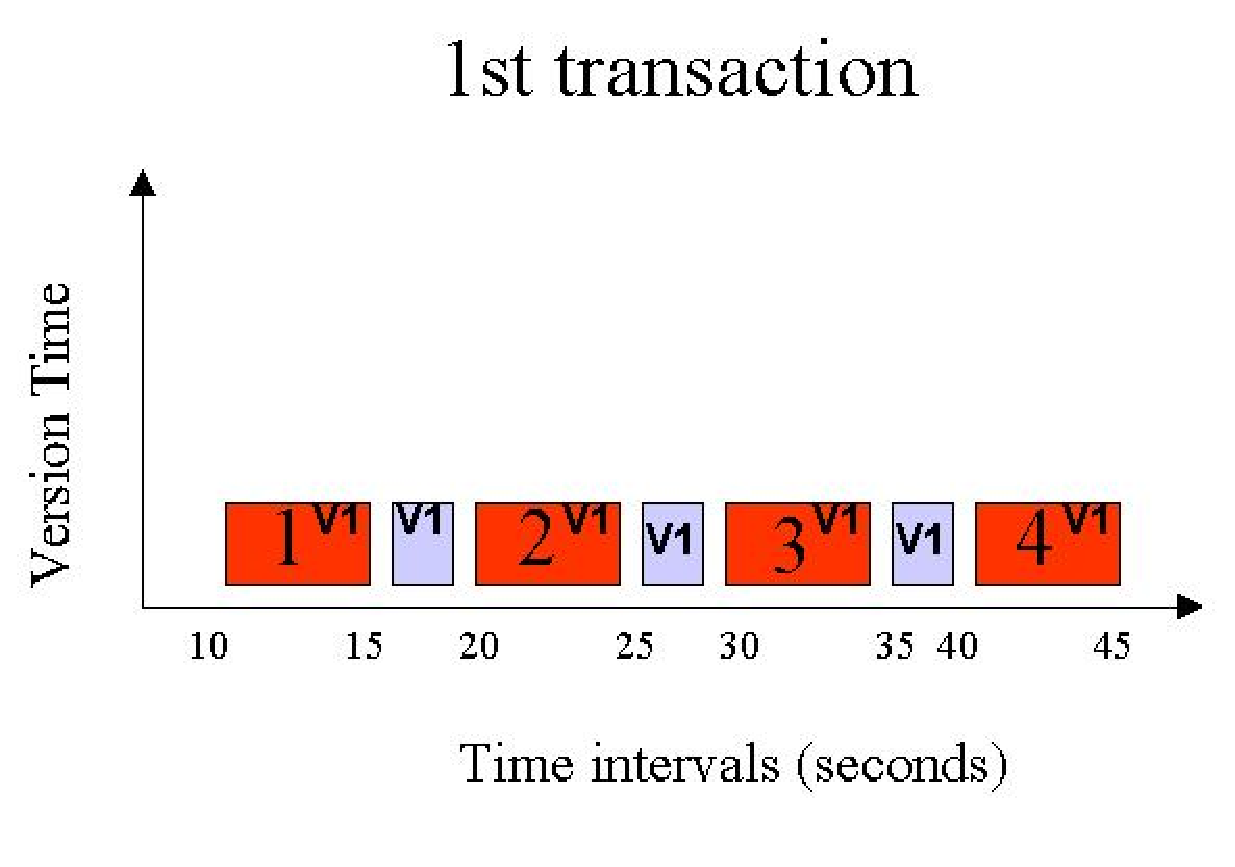
\includegraphics[width=.7\linewidth, scale=.5]{trans1}

\par

We now add a new calibration, valid for the period covered
by the first two entries created above, as well as the period between them.

\begin{verbatim}
// 2nd run, version the first two intervals 
  calibApp->startUpdate(); 
  theDatabase = new HepCalibDatabase ( calibApp, "cal", dbPathName); 
  theDatabase->open (); 
  
  thePedestalCalData = new ( theDatabase->hint() ) PedestalCal(5); 
  cout << "the object created is " << thePedestalCalData->i <<endl; 
  theBeginTime = HepTime( 1996, 1, 1, 0, 0,  10 ); 
  theEndTime =  HepTime( 1996, 1, 1, 0, 0, 25 ); 
  theDatabase->store ( thePedestalCalData, "PedestalCalCont", theBeginTime,theEndTime, 0 ); 
  theDatabase->close( ); 
  calibApp->commit( ); 
\end{verbatim}

\par

The database now has the following structure:
\par

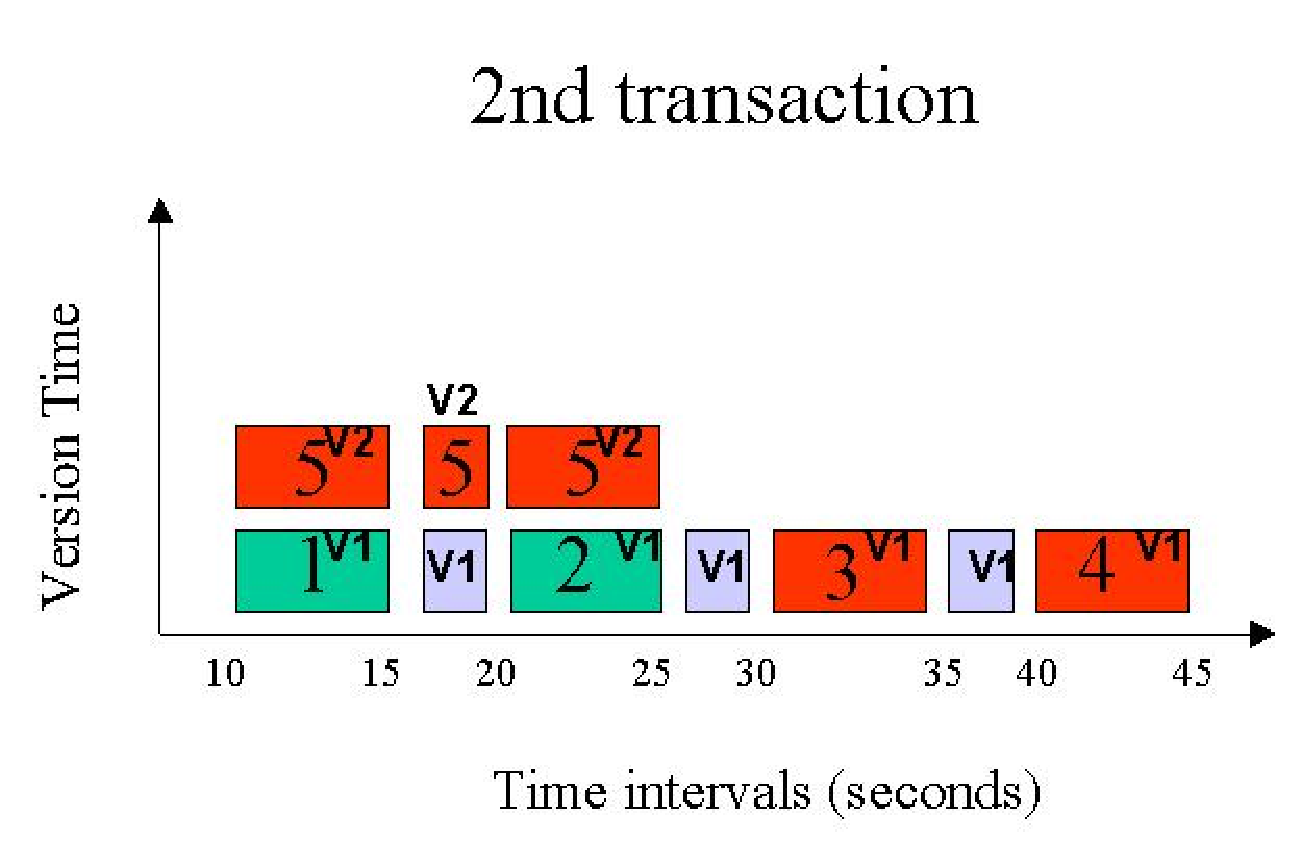
\includegraphics[width=.7\linewidth, scale=.5]{trans2}

\par

We now add a new calibration, valid for the period of the third calibration
created in the first step.
\begin{verbatim}
// 3rd run, version the third interval 
  calibApp->startUpdate(); 
  theDatabase = new HepCalibDatabase ( calibApp, "cal", dbPathName); 
  theDatabase->open (); 
  thePedestalCalData = new ( theDatabase->hint() ) PedestalCal(6); 
  cout << "the object created is " << thePedestalCalData->i <<endl; 
  theBeginTime = HepTime( 1996, 1, 1, 0, 0,  30 ); 
  theEndTime =  HepTime( 1996, 1, 1, 0, 0, 35 ); 
  theDatabase->store ( thePedestalCalData, "PedestalCalCont", theBeginTime,theEndTime, 0 ); 
  theDatabase->close( ); 
  calibApp->commit( ); 
\end{verbatim}

\par

The database structure now looks as follows:
\par

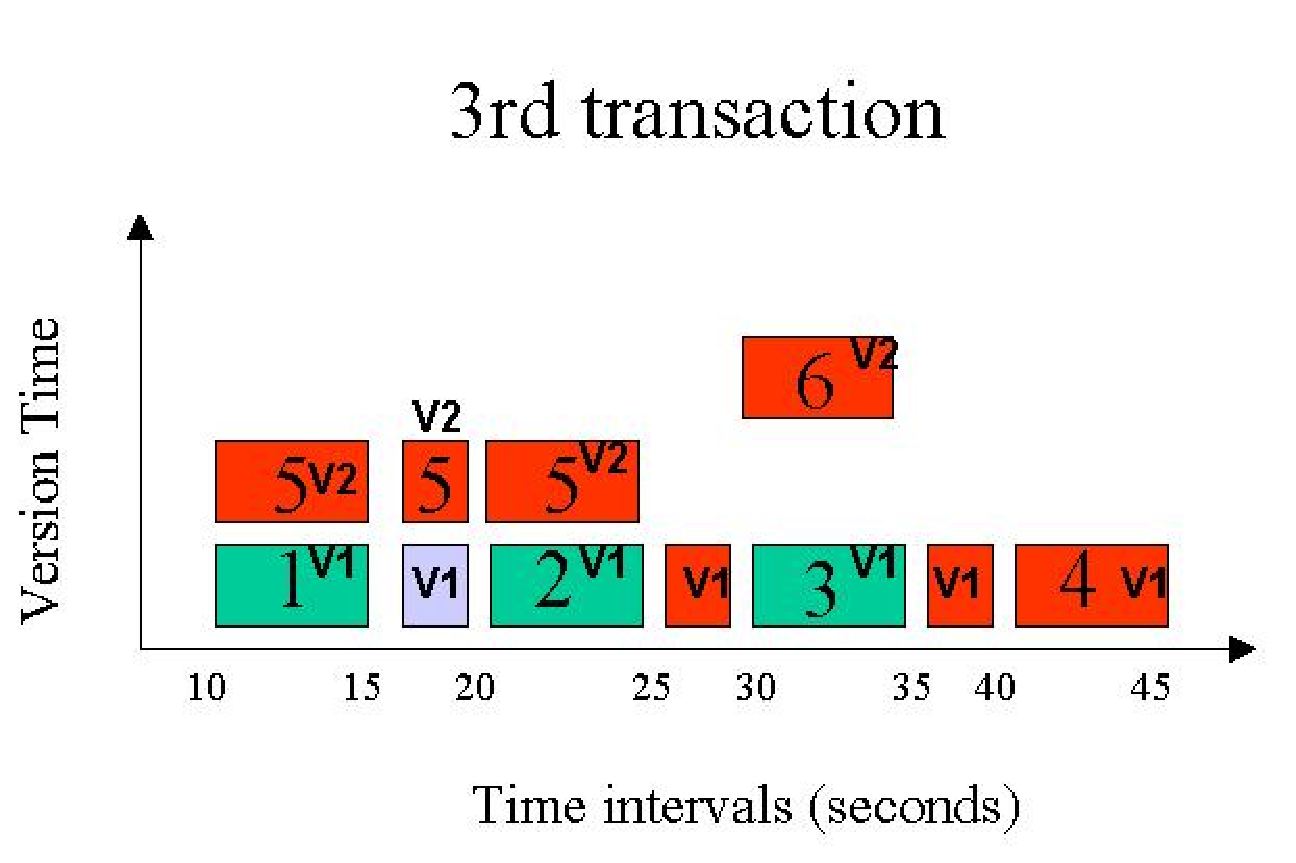
\includegraphics[width=.7\linewidth, scale=.5]{trans3}

\par

We now add yet further calibrations, demonstrating how an existing validity period can
be subdivided.
\begin{verbatim}
// 4th run, split the value of one interval 
  calibApp->startUpdate(); 
  theDatabase = new HepCalibDatabase ( calibApp, "cal", dbPathName); 
  theDatabase->open (); 
  thePedestalCalData = new ( theDatabase->hint() ) PedestalCal(7); 
  cout << "the object created is " << thePedestalCalData->i <<endl; 
  theBeginTime = HepTime( 1996, 1, 1, 0, 0,  42 ); 
  theEndTime =  HepTime( 1996, 1, 1, 0, 0, 43 ); 
  theDatabase->store ( thePedestalCalData, "PedestalCalCont", theBeginTime,theEndTime, 0 ); 
  theDatabase->close( ); 
  calibApp->commit( ); 
\end{verbatim}

\par

The database structure now looks like:
\par

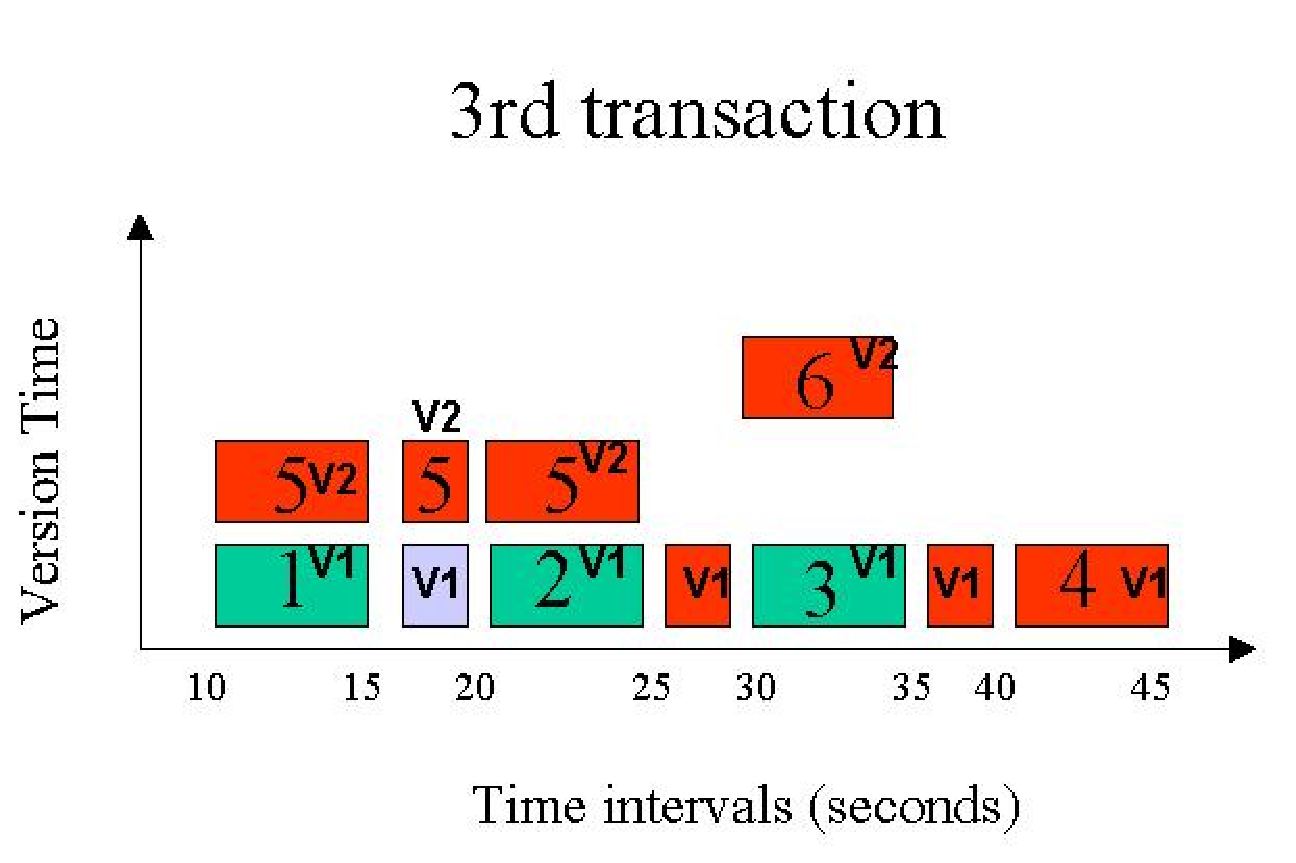
\includegraphics[width=.7\linewidth, scale=.5]{trans3}

\par

The following example shows retrieval by validity instant and handling of versions.

\begin{verbatim}
//File:/HepODBMS/examples/readCalibration/readCalibration.cpp 
  
calibApp->startRead (); 
theDatabase = new HepCalibDatabase ( calibApp, "cal", dbPathName);

  
  // open the cal DB 
  theDatabase->open (); 
  // define the interval you look for 
  theBeginTime = HepTime( 1996, 1, 1, 0, 0,  20 ); 
  
  // Find the interval corresponding to theTime 
  // findInterval( BdbIntervalH, theContainerName, anyTime, atag ) 
  HepRef(calibInterval) theInterval; 
  int res = theDatabase->findInterval( theInterval, "PedestalCalCont", theBeginTime ); 
  if (res) 
  { 
    cout << "the interval was found" << endl; 
    HepRef( PedestalCal ) thePedestalCalDataFound =(HepRef(PedestalCal)) theInterval->getObject( ); 
    if (thePedestalCalDataFound != 0 ) { 
      HepTime theVersionTime = theInterval -> getVersionTime( ); 
      cout << "the object found had a pedestal of: " << thePedestalCalDataFound->i <<endl; 
    } 
  } 
  else 
 cout << "the interval was not found" << endl; 

  // get version name of this interval 
  char * version; 
  version = new char [3]; 
  version = theInterval->getVersionNumber(); 
  cout << "Version number of the interval found : " << version << endl; 
  
  
  // get V1 from this interval 
  HepRef( calibInterval ) intervalFoundH; 
  intervalFoundH = theInterval->getCalibInterval( "v1" ); 
  if ( intervalFoundH != 0 ) 
  { 
    cout << "the interval with version V1 was found" << endl; 
    HepRef( PedestalCal ) thePedestalCalDataFound =(HepRef(PedestalCal)) intervalFoundH->getObject( ); 
    if (thePedestalCalDataFound != 0 ) { 
      HepTime theVersionTime = intervalFoundH -> getVersionTime( ); 
      cout << "the object found had a pedestal of: " << thePedestalCalDataFound->i <<endl; 
    } 
  } 
  else 
 cout << "the interval with version v1 does not exist" << endl; 
  

  // read previous values (versions) of the interval found 
  cout << "reading all version values of this interval " << endl; 
  HepRef( calibInterval ) prevH,intervalH; 
  if ( ( theInterval->hasVersion() ) && ( theInterval !=0 ) ) 
    { 
      theInterval->prevVers( prevH ); 
      intervalH = prevH; 
      while ( intervalH != 0 ) 
 { 
   HepRef( PedestalCal ) thePedestalCalDataFound =(HepRef(PedestalCal)) intervalH->getObject( ); 
   if ( thePedestalCalDataFound != 0 ) 
     cout << "previous version value: " << thePedestalCalDataFound->i <<endl; 
   intervalH->prevVers ( prevH ); 
   intervalH = prevH; 
 } 
    } 
  else 
    cout << "has no versions. " << endl; 

  // read the default version from minus infinite to infinite 
  cout << " reading the current default version for Pedestal ... " << endl; 
  theDatabase->firstInterval( intervalH, "PedestalCalCont" ); 
  while ( (intervalH = intervalH->next( )) != 0 ) 
  { 
     cout << intervalH << endl; 
     HepRef(PedestalCal) thePedestalCalDataFound = (HepRef(PedestalCal))intervalH->getObject( ); 
     if (thePedestalCalDataFound != 0 ) 
   cout << "- Pedestal value: " << thePedestalCalDataFound->i <<endl; 
     else 
       cout << "- Pedestal value: EMPTY" << endl; 
  
  } 
  theDatabase->close( ); 
\end{verbatim}

\par

The following example shows the definition of a trivial
(non-realistic) calibration class.  The class is made persistent by
inheritence (from \Lit{HepPersObjy}. The \Lit{HepTime}
class is made persistent by containment.
\begin{verbatim}
//File:/HepODBMS/examples/readCalibration/PedestalCal.ddl

#ifndef pedestalcal.ddl 
#define pedestalcal.ddl 
#include "HepODBMS/odbms/HepODBMS.h" 
class HepTime; 
  
class PedestalCal : public HepPersObj { 
public: 
  
  int i; 
  // constructors 
  PedestalCal() {i=0;}; 
  PedestalCal(int a) {i = a;} ; 

  // set and get function 
  void set_PedestalCal(int a) {i=a;}; 
  int get_PedestalCal( ) {return i;}; 
  
}; 
\end{verbatim}
\section{Conditions DB Examples}

\par

In order to run the calibration database examples, follow the instructions for running
HepODBMS examples for Unix or NT as appropriate. For example, the \Lit{readCalibration}
example contains:\begin{DLtt}{readCalibration.cpp}
\item[Pedestal.ddl]The calibration type definition for pedestal
\item[readCalibration.cpp]The main function. It will start six transactions to store and read the calibrations.
\item[GNUmakefile]The makefile to copy the federeated database and schema from HepODBMS, compile and link readCalibration.
\item[example_setup]Script to set the environment variables to run the program
\end{DLtt}

\par

Having built the example, set the boot file and location of the calibration
database files as appropriate:
\begin{alltt}

setenv OO_FD_BOOT \emph{your local directory}/readCalibration/db/calibration 
setenv OO_DB_PATH \emph{your local directory}/readCalibration/db 
 \emph{your local directory}/readCalibration/readCalibration 

\end{alltt}

\par

The following output will be produced.
\begin{verbatim}
%source example_setup ( should set OO_FD_BOOT,  OO_DB_PATH and LD_LIBRARY_PATH(in UNIX)or PATH (in NT) ) 
%readCalibration: 
WARNING: HepDbApplication: Could not find naming root directory: Naming will be disabled. 
the object created is 1 
the object created is 2 
the object created is 3 
the object created is 4 
the object created is 5 
the object created is 6 
the object created is 7 
the interval was found 
the object found had a pedestal of: 5 
Version number of the interval found : V1 
the interval with version V1 was found 
the object found had a pedestal of: 5 
reading all version values of this interval 
previous version value: 2 
 reading the current default version for Pedestal ... 
* Calibration Interval: 
- beginTime: 01/01/96 01:00:10:000000GMT, nanoseconds: 0 
- endTime: 01/01/96 01:00:15:000000GMT, nanoseconds: 0 
- version time: 04/23/99 19:18:48:000000GMT, nanoseconds: 0 
- tag: 0 
- Pedestal value: 5 
* Calibration Interval: 
- beginTime: 01/01/96 01:00:15:000000GMT, nanoseconds: 0 
- endTime: 01/01/96 01:00:20:000000GMT, nanoseconds: 0 
- version time: 04/23/99 19:18:49:000000GMT, nanoseconds: 0 
- tag: 0 
- Pedestal value: 5 
* Calibration Interval: 
- beginTime: 01/01/96 01:00:20:000000GMT, nanoseconds: 0 
- endTime: 01/01/96 01:00:25:000000GMT, nanoseconds: 0 
- version time: 04/23/99 19:18:49:000000GMT, nanoseconds: 0 
- tag: 0 
- Pedestal value: 5 
* Calibration Interval: 
- beginTime: 01/01/96 01:00:25:000000GMT, nanoseconds: 0 
- endTime: 01/01/96 01:00:30:000000GMT, nanoseconds: 0 
- version time: 04/23/99 19:18:48:000000GMT, nanoseconds: 0 
- tag: 0 
- Pedestal value: EMPTY 
* Calibration Interval: 
- beginTime: 01/01/96 01:00:30:000000GMT, nanoseconds: 0 
- endTime: 01/01/96 01:00:35:000000GMT, nanoseconds: 0 
- version time: 04/23/99 19:18:50:000000GMT, nanoseconds: 0 
- tag: 0 
- Pedestal value: 6 
* Calibration Interval: 
- beginTime: 01/01/96 01:00:35:000000GMT, nanoseconds: 0 
- endTime: 01/01/96 01:00:40:000000GMT, nanoseconds: 0 
- version time: 04/23/99 19:18:48:000000GMT, nanoseconds: 0 
- tag: 0 
- Pedestal value: EMPTY 
* Calibration Interval: 
- beginTime: 01/01/96 01:00:40:000000GMT, nanoseconds: 0 
- endTime: 01/01/96 01:00:42:000000GMT, nanoseconds: 0 
- version time: 04/23/99 19:18:51:000000GMT, nanoseconds: 0 
- tag: 0 
- Pedestal value: 4 
* Calibration Interval: 
- beginTime: 01/01/96 01:00:42:000000GMT, nanoseconds: 0 
- endTime: 01/01/96 01:00:43:000000GMT, nanoseconds: 0 
- version time: 04/23/99 19:18:51:000000GMT, nanoseconds: 0 
- tag: 0 
- Pedestal value: 7 
* Calibration Interval: 
- beginTime: 01/01/96 01:00:43:000000GMT, nanoseconds: 0 
- endTime: 01/01/96 01:00:45:000000GMT, nanoseconds: 0 
- version time: 04/23/99 19:18:51:000000GMT, nanoseconds: 0 
- tag: 0 
- Pedestal value: 4 
* Calibration Interval: 
- beginTime: 01/01/96 01:00:45:000000GMT, nanoseconds: 0 
- endTime: +Infinity 
- version time: 04/23/99 19:18:48:000000GMT, nanoseconds: 0 
- tag: 0 
- Pedestal value: EMPTY 
\end{verbatim}

\par

The datbase contents may be viewed using:
\begin{itemize}

\item oobrowse ./db/Calibration (in NT ) 
\item ootoolmgr  ./db/Calibration  (in UNIX ) \end{itemize}
\chapter{Examples\label{H1Examples}}
\section{Running the Examples on Unix}

\par

In this section, we describe how you may run the HepODBMS example programs.
We describe the procedure for the \Lit{populateDB} example. Exactly
the same procedure may be used for all other examples, simply by using the 
appropriate example name.

\par

Before running the examples, make sure that your environment is correctly configured.
Instructions for running Objectivity/DB either from \Lit{AFS} or for installing locally
are available \url{http://wwwinfo.cern.ch/asd/lhc++/Objectivity/index.html}.

\par

In particular, you should check that the following two environment variables
are correctly set.
\begin{itemize}

\item OBJY_DIR
\item LD_LIBRARY_PATH(or equivalent)\end{itemize}

\par

It is also recommended that you run the examples in \Lit{standalone} mode. As shown in
the following diagram, this means that neither data server (AMS) nor lockserver are required.
\par

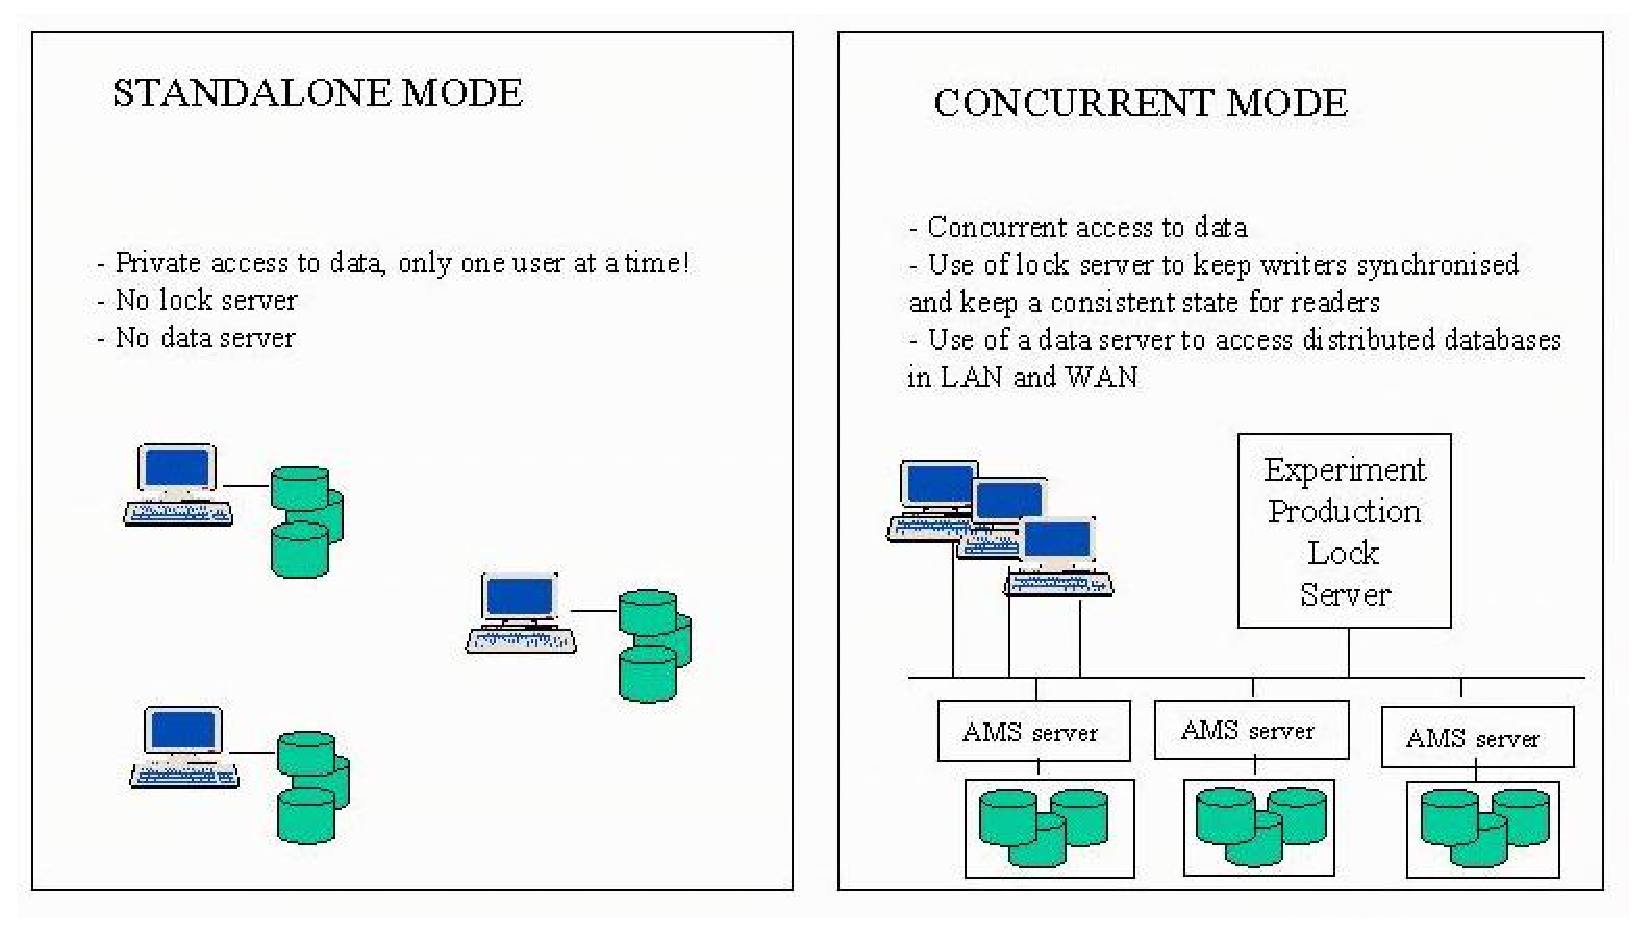
\includegraphics[width=.7\linewidth, scale=.5]{sa-vs-ls}

\par
\Lit{Do not run in standalone mode against a production federation} (or indeed
any other federation that is shared).
\par

To run in standalone mode, set the \Lit{STANDALONE}environment variable as follows:
\begin{verbatim}
# C shell
setenv STANDALONE 1
\end{verbatim}

\begin{verbatim}
# Bourne Shell: 
STANDALONE=1 
export STANDALONE 
\end{verbatim}

\par

Add the following code to your application just before you call the
database initialization function, i.e. before calling the constructor 
of \Lit{HepDbApplication} or \Lit{HepCalibApplication}:
\begin{verbatim}
#ifdef nolockserver 
  ooNoLock(); 
#endif
\end{verbatim}

\par

You should now copy the examples to your local directory, as follows:
\begin{alltt}

cp -r /afs/cern.ch/sw/lhcxx/share/HepODBMS/new/examples/populateDb \emph{your local directory}
\end{alltt}

\par

You will now have the following files:\begin{DLtt}{SimpleTrackTable.ddl}
\item[Event.ddl]DDL file to define the persistent Event type
\item[GNUmakefile]The makefile for the example
\item[SimpleTrackTable.ddl]DDL file to define persistent the Track Table
\item[example_setup]Script to perform the setup of the environment variables
\item[populateDb.cpp]The main program
\item[randomSource.cpp]Source file and...
\item[randomSource.h]header file to generate random tracks and clusters
\end{DLtt}

\par

The \Lit{example_setup} file is as follows:
\begin{verbatim}
HEP_ODBMS_DIR=/afs/cern.ch/sw/lhcxx/specific/$OS/HepODBMS/new 
export HEP_ODBMS_DIR 
#STANDALONE=1   TAKE THE COMMENT OUT IF YOU WORK IN STANDALONE MODE 
#export STANDALONE 
OO_FD_BOOT=`pwd`/db/EXAMPLE_FD 
export OO_FD_BOOT 
LD_LIBRARY_PATH=/afs/cern.ch/sw/lhcxx/specific/$OS/HepODBMS/new/lib:$LD_LIBRARY_PATH 
\end{verbatim}

\par

Edit this file as appropriate.
\par

Once correctly configured, \emph{source} the file.
\begin{verbatim}
source example_setup # C shell

%  vi GNUmakefile EDIT GNUmakefile and add schema in path 
"$(HEP_ODBMS_DIR)"/etc/getdb $(HEP_ODBMS_DIR)/schema/HEP_BASE $(BOOT) ${FDID}
%  gmake VERBOSE=1 
\end{verbatim}

\par

This makefile does automatically all steps needed to create the federated database, load the schema and make the executable: 

\begin{itemize}

\item creates a platform specific directory where the object files
will be located: LINUX, Solaris.. 
\item copies the \Lit{HEP-BASE} federated database from
HepODBMS and installs it in your local subdirectory
\Lit{~HepODBMS/examples/populatedb/db} with the name
\Lit{EXAMPLE_FD}. If you are in \Lit{STANDALONE} mode
you should \emph{only} access your private federated
database
\item runs the \Lit{ooddlx} preprocessor on all schema files
(\Lit{*.ddl}) and generates \Lit{.h},
\Lit{_ref.h}, and \Lit{_ddl.cpp} files.
\item compiles and links the \Lit{populateDb} application with
the schema files and produces the executable.\end{itemize}

\par

The example may now be run as shown below.
\begin{verbatim}
[pc30] ~/examples/populateDb % populateDb 10 # Generate 10 events
*** starting execution of populateDb 
*** about to initialise the database session 
WARNING: HepDbApplication: Could not find naming root directory: Naming will be disabled. 
*** creating 10 Events ... done. 
*** generated 100 tracks and 100 clusters in total. 
[pc30] ~/examples/populateDb %
\end{verbatim}

\par
\Lit{N.B.}If you run your application in \Lit{STANDALONE}
mode you should use the \Lit{-standalone} when using any of the Objectivity/DB tools.
For example, to view the objects using the \Lit{ootoolmgr} tool, use:

\begin{verbatim}
% examples/populateDb > ootoolmgr [-standalone] ./db/EXAMPLE_FD 
\end{verbatim}

\par

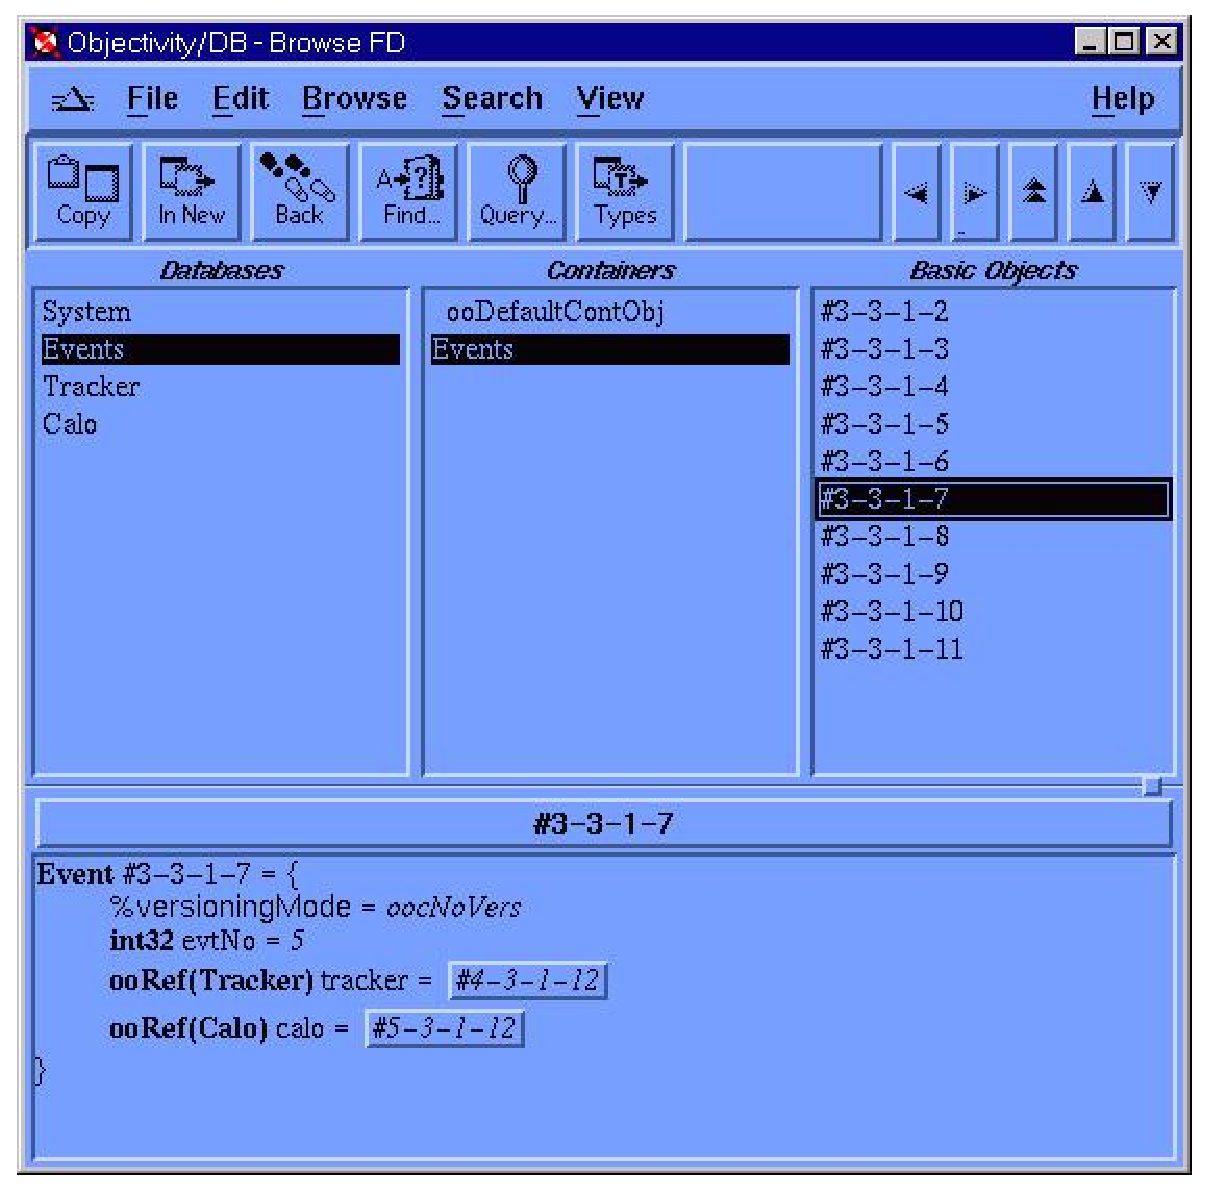
\includegraphics[width=.7\linewidth, scale=.5]{ootoolmgr}

\par

Alternatively, you may
simply run the \Lit{oodump} tool, which will dump the database in raw text format
as follows: 

\begin{verbatim}
 % examples/populateDb > oodump [-standalone] -db TrackData ./db/EXAMPLE_FD 
\end{verbatim}

\par

You can check also the database catalog of the \Lit{EXAMPLE_FD} federated database as follows:
\begin{verbatim}
% examples/populateDb > oodumpcatalog [-standalone] ./db/EXAMPLE_FD 
\end{verbatim}

\par

In standalone mode, this would produce something like the following.
\begin{verbatim}
/populateDb/db % oodumpcatalog -standalone EXAMPLE_FD 
Objectivity/DB (TM) List Database Files Utility, Version 5.1.0 
Copyright (c) Objectivity, Inc 1990, 1998. All rights reserved. 

FD Name   = EXAMPLE_FD 
FD ID     = 1 
FD File   = pc30::/populateDb/db/EXAMPLE_FD.FDDB 
Boot File = pc30::/populateDb/db/EXAMPLE_FD 
Jnl Dir   = pc30::/populateDb/db 
Lock Host = GHOST (lockserver is set to GHOST automatically if you run in standalone mode) 

DB Name   = System 
DB ID     = 2 
DB Image  = pc30::/populateDb/db/System.EXAMPLE_FD.DB 

DB Name   = Events 
DB ID     = 3 
DB Image  = pc30::/populateDb/db/Events.EXAMPLE_FD.DB 

DB Name   = Tracker 
DB ID     = 4 
DB Image  = pc30::/populateDb/db/Tracker.EXAMPLE_FD.DB 

DB Name   = Calo 
DB ID     = 5 
DB Image  = pc30::/populateDb/db/Calo.EXAMPLE_FD.DB 

/populateDb/db

\end{verbatim}
\section{Running the Examples on NT}

\par

Before running the examples, ensure that both Objectivity/DB and ObjectSpace are installed.
Instructions on installing Objectivity/DB locally can be found via the following URL:
\url{http://wwwinfo.cern.ch/asd/lhc++/Objectivity/index.html}.

\par

You then need to install the GNU tools (CYGWIN-B20.1), available via
the following URL: \url{http://sourceware.cygnus.com/cygwin/}. These tools are ports
of the popular GNU development tools and utilities for Windows 95, 98,
and NT.  Using the GNU tools you will start a bash shell and proceed
as in UNIX, the only difference being the settings for the
\Lit{HEP_ODBMS_DIR} and \Lit{OBJY_DIR} environment
variables.

\begin{alltt}

ALL STEPS YOU HAVE TO DO TO RUN WITH GNU TOOLS: 
  
bash-2.02$ \Ucom{cp -r z:/P32/lhcxx/share/HepODBMS/new/HepODBMS/examples/populateDb . }
bash-2.02$ \Ucom{cd populateDb}
bash-2.02$ \Ucom{vi GNUmakefile} (Edit GNUmakefile) 
   getdb $(HEP_ODBMS_DIR)/schema/HEP_BASE $(BOOT) ${FDID} 
bash-2.02$ \Ucom{vi example_setup} (edit example_setup as it follows) 
#!/bin/sh 
HEP_ODBMS_DIR=z:/P32/lhcxx/specific/Windows_NT/HepODBMS/new 
export HEP_ODBMS_DIR 
OBJY_DIR=d:/objy51 (set your local path!) 
export OBJY_DIR 
#STANDALONE=1 (TAKE COMMENT ONLY IF YOU RUN IN STANDALONE MODE) 
#export STANDALONE 
OO_FD_BOOT=`pwd`/db/EXAMPLE_FD 
export OO_FD_BOOT 
PATH=z:/P32/lhcxx/specific/Windows_NT/HepODBMS/new/lib:$PATH 
export PATH
bash-2.02$ \Ucom{source example_setup}
bash-2.02$ \Ucom{gmake} ( you can use VERBOSE=1 ) 
WARNING: LHCXXTOP is not defined! [z:/p32/lhcxx will be used] 
WARNING: PLATF is not defined! [ Windows_NT will be used] 
"z:/p32/lhcxx/specific/windows_NT/HepODBMS/new"/etc/getdb z:/p32/lhcxx/specific/ 
windows_NT/HepODBMS/new/schema/HEP_BASE db/EXAMPLE_FD 1 
ATTENTION:getdb in STANDALONE MODE 
Schema import from HEP_BASE to EXAMPLE_FD 
Updating Name Service values... 
Now updating System Name Space (catalog) values... 
Now updating Database File locations... 

Federated Database Installation complete. 
generating schema for Event 

compiling Event_ddl 
Event_ddl.cpp 
compiling populateDb 
populateDb.cpp 
compiling randomSource 
randomSource.cpp 
Linking ...

bash-2.02$ \Ucom{populateDb 10} 
*** starting execution of populateDb 
*** about to initialise the database session 
WARNING: HepDbApplication: Could not find naming root directory: Naming will be 
disabled. 
*** creating 10 Events ... done. 
*** generated 100 tracks and 100 clusters in total. 
note: if you run in standalone mode remember to have following code in 
your populateDb.cpp, if not it will not run: 

      #ifdef nolockserver 
              ooNoLock(); 
      #endif 
      app.init("db/EXAMPLE_FD"); 

\end{alltt}

\par

We can now generate a catalog of the database content as follows.

\begin{alltt}

bash-2.02$ \Ucom{oodumpcatalog -standalone db/EXAMPLE_FD}
\end{alltt}

\begin{verbatim}
Objectivity/DB (TM) List Database Files Utility, Version 5.1.0 
Copyright (c) Objectivity, Inc 1990, 1998. All rights reserved. 
FD Name   = EXAMPLE_FD 
FD ID     = 1 
FD File   = pc20::D:\populateDb\db\EXAMPLE_FD.FDDB 
Boot File = pc20::D:\populateDb\db\EXAMPLE_FD 
Jnl Dir   = pc20::D:\populateDb\db 
Lock Host = GHOST 

DB Name   = System 
DB ID     = 2 
DB Image  = pc20::D:\populateDb\db\System.EXAMPLE_FD.DB 

DB Name   = Events 
DB ID     = 3 
DB Image  = pc20::D:\populateDb\db\Events.EXAMPLE_FD.DB 

DB Name   = Tracker 
DB ID     = 4 
DB Image  = pc20::D:\populateDb\db\Tracker.EXAMPLE_FD.DB 

DB Name   = Calo 
DB ID     = 5 
DB Image  = pc20::D:\populateDb\db\Calo.EXAMPLE_FD.DB 

\end{verbatim}

\par

The database browser allows you to obtain a pictural
representation as follows.
\begin{alltt}

bash-2.02$ \Ucom{oobrowse -standalone db/EXAMPLE_FD}
\end{alltt}

\par

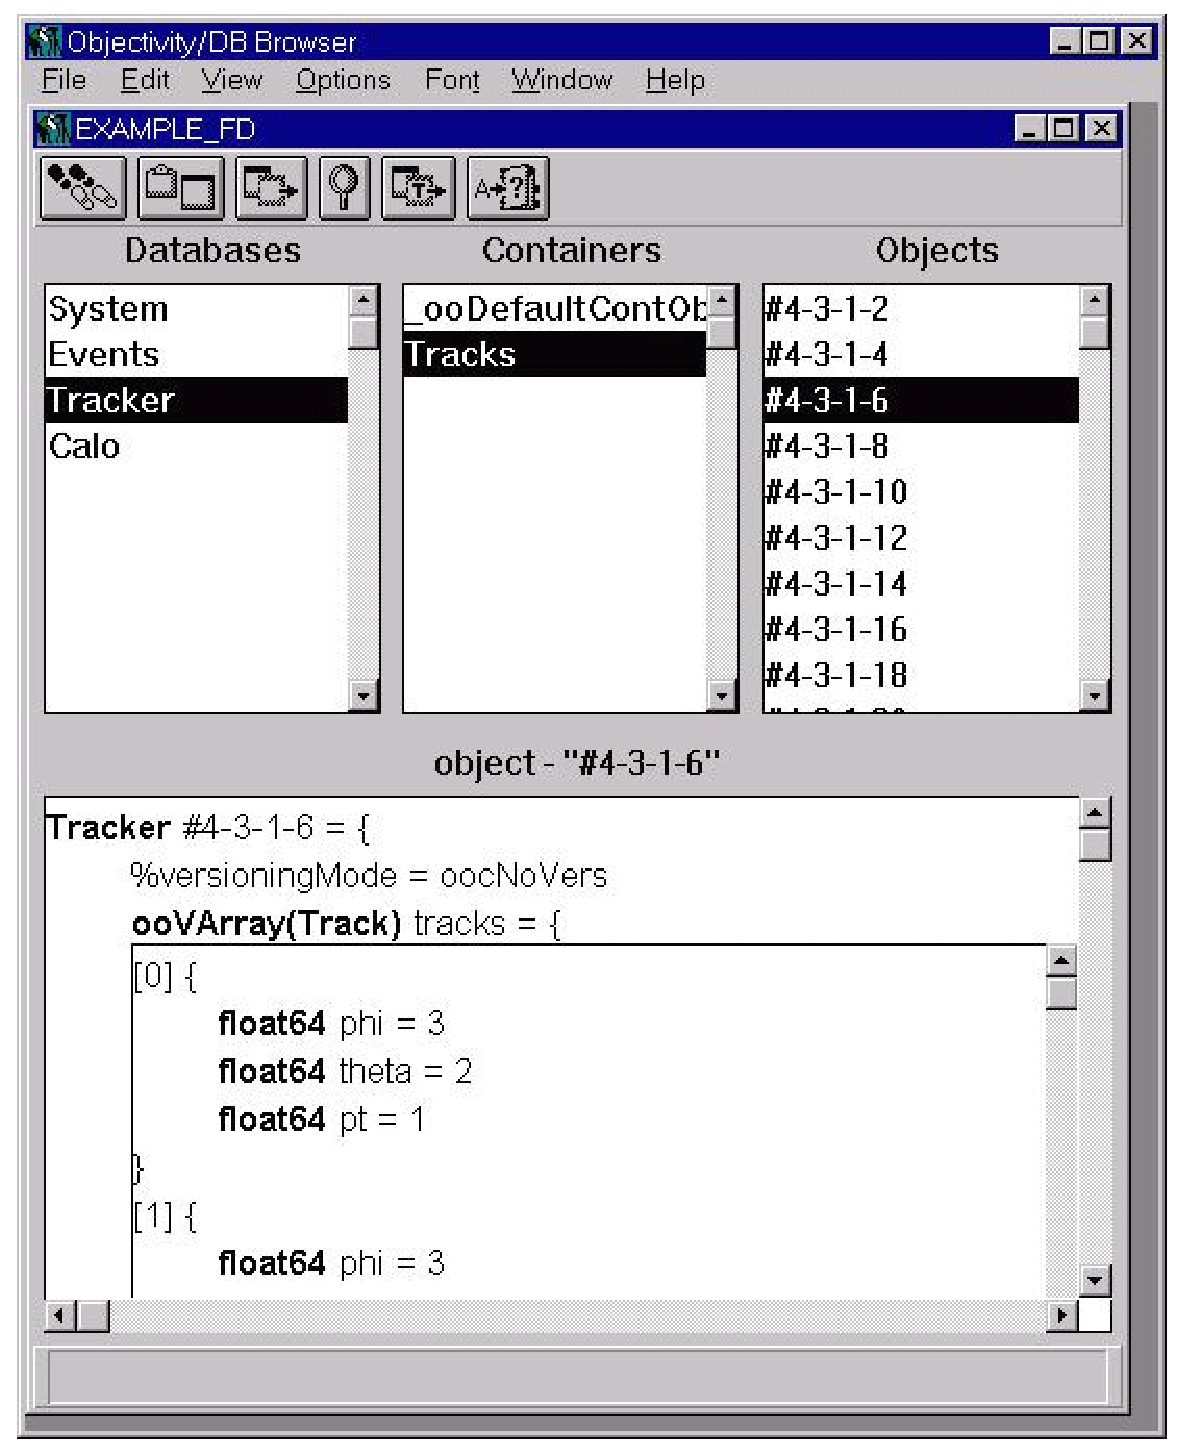
\includegraphics[width=.7\linewidth, scale=.5]{oobrowse}

\appendix
